\documentclass[12pt,journal,onecolumn,draftclsnofoot]{IEEEtran}
\usepackage[T1]{fontenc}
\usepackage[utf8]{inputenc}
\usepackage{cite}
\usepackage{url}
\usepackage{booktabs}
\usepackage{longtable}
\usepackage{tabularx}
\usepackage{array}
\usepackage{enumitem}
\usepackage{listings}
\usepackage{tikz}
\usetikzlibrary{arrows.meta,positioning,fit,shapes.geometric,calc}
\usepackage{amsmath,amssymb}
\usepackage[hidelinks]{hyperref}
\usepackage{geometry}
\geometry{margin=0.85in}
\setlist[itemize]{leftmargin=*,itemsep=2pt,topsep=2pt}
\setlist[enumerate]{leftmargin=*,itemsep=2pt,topsep=2pt}
\lstset{basicstyle=\ttfamily\scriptsize,breaklines=true,columns=fullflexible,frame=single,keepspaces=true}
\newcolumntype{Y}{>{\raggedright\arraybackslash}X}
\sloppy

\title{JCP/1.0.0 and the Joint Master Control Plane: A Protocol-First Supervisory Architecture for Autonomous Engineering, Minimal User Attention, and Governed Self-Improvement}
\author{Prepared for Jepson Taylor and the NEVERHUMAN JMCP Program\\June 2026}
\begin{document}
\maketitle

\begin{abstract}
Autonomous engineering systems are moving from single coding assistants toward persistent ecosystems of agents, tools, repositories, memories, continuous integration systems, and production pathways. The limiting problem is no longer whether a model can act, but whether a supervisory system can decide what should be acted upon, who or what may act, what authority is granted, what evidence is required, what the user must see, and what must be blocked. This paper defines the Joint Master Control Plane (JMCP) and freezes JCP/1.0.0, the Joint Control Protocol that all services, tools, agents, data adapters, text interfaces, and voice gateways must use to communicate with JMCP. JCP/1.0.0 specifies signed envelopes, ServiceCards, ToolCards, DataCards, AgentCards, WorkOrders, Tasks, CapabilityLeases, ContextContracts, EvidenceBundles, AttentionPackets, VoiceTurns, MemoryProposals, SelfImprovementProposals, ToolBuildProposals, PolicyDecisions, PromotionDecisions, FaultReports, telemetry signals, and conformance reports. The design is critique-hardened: it treats agents as untrusted workers, evidence as a promotion requirement rather than a log stream, memory as a governed proposal pipeline, and user attention as a scarce safety-critical resource. The final architecture positions JMCP above MCP, A2A, CI, observability, agent frameworks, and workflow engines. It uses those systems, but does not delegate authority, evidence, memory, or user-attention governance to them.
\end{abstract}

\begin{IEEEkeywords}
agentic AI, control plane, model context protocol, software engineering automation, observability, capability security, evidence, provenance, voice interface, self-improvement, tool building.
\end{IEEEkeywords}

\section{Introduction}
Software engineering is entering a transition from assistant-mediated work to delegated work. A user no longer wants to manage every log, issue, branch, build, tool, model, and agent. The user wants to state intent sparsely, remain informed about meaningful decisions, and trust the system to investigate, route, constrain, verify, and improve. The challenge is not only automation. It is control observability, security, task governance, memory governance, evidence, and value optimization.

The Joint Master Control Plane (JMCP) is designed for that transition. JMCP is the primary user interface and supervisory authority for autonomous engineering. It accepts text and voice intent, decomposes work into controlled tasks, leases capability to subordinate systems, supervises tools and agents, gathers evidence, promotes only proof-carrying outputs, and decides what must be surfaced to the user. It protects the user from excessive information without hiding important decisions.

The prior JMCP drafts correctly identified the central idea: JMCP should not be ``the agent.'' It should be the authority, evidence, and process-control layer above agents. However, a final design needs more than a strong concept. It needs a mandatory protocol. Every program, service, tool, datastore adapter, agent, text surface, and voice gateway must communicate through one versioned standard. Without that standard, the system degenerates into undocumented webhooks, hidden side channels, brittle adapters, untracked authority, inconsistent task state, and evidence theater.

This paper freezes the final naming and protocol boundary. \textbf{JMCP} is the product and supervisory control plane. \textbf{JCP/1.0.0} is the wire-level Joint Control Protocol. \textbf{JPCM} is the recommended communication backbone profile that transports JCP envelopes, typically through durable event streams, request/reply, replay, and interactive streaming. The protocol is intentionally stricter than a general tool protocol or agent-to-agent protocol because JMCP's purpose is not only interoperability. It is authority, evidence, attention, and safe autonomy.

\section{Contributions}
This paper makes five contributions.

First, it provides a negative definition: JMCP is not a chatbot, MCP host, A2A peer, CI dashboard, log viewer, task queue, or agent framework. It may use all of those, but it owns the authority boundary above them.

Second, it defines JCP/1.0.0 as a mandatory protocol for all communication with JMCP. JCP includes a signed envelope, canonical message families, service identity, policy epoch, capability leases, data classification, evidence references, trace context, and payload schemas.

Third, it defines a complete object model for autonomous engineering work: intents, work orders, tasks, leases, context contracts, service cards, tool cards, data cards, agent cards, evidence bundles, attention packets, voice turns, memory proposals, self-improvement proposals, automated tool-building proposals, policy decisions, promotion decisions, faults, telemetry, and conformance reports.

Fourth, it converts the strongest criticisms of prior drafts into hard requirements: no side effect without lease, no promotion without evidence, no durable memory without proposal and contradiction checks, no irreversible voice action without confirmation, no self-improvement that silently changes authority, and no service authority without conformance.

Fifth, it defines the future vector: JMCP can evolve from an engineering command room into an autonomous engineering fab, cross-repository yield optimizer, engineering digital twin, autonomous R\&D foundry, proof-carrying agent economy, and federated trust mesh.

\section{Hostile Review of the Prior Corpus}
A final architecture must survive hostile review. The uploaded V5 bundle contained multiple V4 engineering specifications, white papers, and schema seeds. Their common strengths were clear: they understood that JMCP is an authority layer, not another agent; they emphasized evidence and user attention; and they correctly placed Jankurai, Jeryu, and Jekko below JMCP as specialized subsystems. Their common weaknesses were also clear.

\subsection{Naming Drift}
The corpus used JMCP, JPMC, JPCM, JPCP, JMCP-CP, and JCP. This is not cosmetic. Protocol naming drift becomes implementation drift. A service cannot conform to a moving name. V5 resolves the names: JMCP is the system, JCP/1.0.0 is the protocol, and JPCM is the backbone profile.

\subsection{Incomplete Schema}
The V4 schemas were envelope seeds, not complete protocol schemas. They did not sufficiently define task types, voice, memory, self-improvement, automated tool building, conformance reports, fault reports, ToolCards, DataCards, AgentCards, or promotion decisions. A final control plane must treat those as first-class objects.

\subsection{Weak Self-Improvement Gates}
The prior drafts correctly wanted JMCP to improve continuously. The dangerous gap was how. Self-improvement can corrupt authority, memory, routing, evidence thresholds, or user-attention filters. V5 requires a SelfImprovementProposal, safety case, evaluation plan, shadow mode, red-team test, promotion decision, and rollback plan.

\subsection{Evidence Theater}
Most drafts said evidence is required, but did not always separate logs from proof. Evidence theater occurs when a system generates impressive artifacts that do not actually support the relevant claim. V5 requires evidence bundles to map evidence to claims, include negative evidence, identify sufficiency level, preserve provenance, and block promotion when evidence conflicts.

\subsection{Attention Failure}
A system designed to share the bare minimum can fail in two opposite ways. It can spam the user with every operational detail, or it can become dangerously quiet. V5 defines the Attention Firewall, attention classes, mandatory escalation triggers, decision packets, and false-quiet tests.

\subsection{Voice Boundary Risk}
Voice is not just an input modality. It is a noisy, spoofable, replayable, ambiguity-prone control channel. V5 treats voice as a first-class protocol family with VoiceTurn objects, transcript confidence, anti-replay nonce, command candidate extraction, and confirmation policy.

\subsection{Tool-Building Ambiguity}
JMCP should build tools, but not through ungoverned self-generated scripts. V5 makes automated tool building a workflow: detect repeated need, propose a tool, write a spec, implement in sandbox, test, fuzz, red-team, shadow, quarantine, promote, monitor, and deprecate.

\section{Scoring Summary}
The full scorecard is delivered separately. Table~\ref{tab:score-summary} summarizes the substantive artifacts.

\begin{longtable}{p{0.38\linewidth}p{0.10\linewidth}p{0.44\linewidth}}
\caption{Summary of hostile review scores.}\label{tab:score-summary}\\
\toprule
Artifact & Score & Main reason \\
\midrule
\endfirsthead
\toprule
Artifact & Score & Main reason \\
\midrule
\endhead
`JMCP\_V4\_ENGINEERING\_SPEC.md` & 81 & Strong laws and future vector; protocol and schema still too thin. \\
`JMCP\_V4\_engineering\_spec(1).md` & 85 & Strong planes and user model; needs stricter rollback and tool-building gates. \\
`jmcp\_v4\_protocol\_first\_engineering\_spec.md` & 89 & Best engineering artifact; still has naming, schema, and formal conformance gaps. \\
`jmcp\_v4\_protocol\_first\_engineering\_spec(1).md` & 86 & Clean protocol-first build, but less complete adversarial and operational depth. \\
`JMCP\_V4\_ieee\_whitepaper.tex` & 78 & Good framing, too thin for final paper. \\
`jmcp\_v4\_ieee\_white\_paper.tex` & 84 & Broad and ambitious, needs tighter protocol semantics. \\
`jmcp\_v4\_protocol\_first\_ieee\_paper.tex` & 87 & Best paper candidate, but below requested final depth. \\
`jmcp\_v4\_whitepaper.tex` & 86 & Broadest white paper, needs a single canonical protocol. \\
`jmcp\_cp\_v1\_envelope.schema.json` & 54 & Useful envelope seed, not complete protocol schema. \\
`jmcp\_v4\_jpcp\_v1\_envelope\_schema.json` & 57 & Slightly better envelope, still incomplete object model. \\
`jmcp\_v4\_scorecard.md` & 80 & Useful critique pressure, not a build spec. \\
\bottomrule
\end{longtable}

\section{Definition: What JMCP Is}
JMCP is a supervisory control plane for autonomous engineering and high-value knowledge work. It receives sparse human intent, constructs work orders, governs tasks, grants limited authority, supervises untrusted workers, requires evidence, learns from results, and controls user attention. JMCP is closer to a fab-level process-control and fault-detection system than to a chatbot. Its primary job is to raise the user's operating altitude.

The system has three important separations. \emph{Authority} is centralized in JMCP and expressed through leases. \emph{Execution} is delegated to tools, agents, scripts, CI systems, and data adapters. \emph{Evidence} is collected independently enough to judge the work. This separation prevents the executor from being the same entity that grants itself authority and certifies its own output.

\section{Definition: What JMCP Is Not}
JMCP is not a chatbot with tools. Chat is one interface, not the architecture. JMCP is not an MCP server; MCP standardizes access to context and tools, while JMCP governs authority, evidence, task state, memory, and user attention. JMCP is not an A2A agent; A2A supports agent interoperability and task communication, while JMCP is the supervising authority. JMCP is not CI; CI generates evidence, but JMCP decides what evidence is required and whether promotion is allowed. JMCP is not a generic agent framework; agents are subordinate workers. JMCP is not a memory system; memory is a governed product of evidence and review.

\section{Related Work and Gap}
MCP provides a standardized way for LLM applications to connect with external data sources and tools through hosts, clients, servers, JSON-RPC messages, resources, prompts, and tools \cite{mcp2025}. Its security guidance emphasizes user consent, data privacy, tool safety, and sampling controls, but also notes that MCP itself cannot enforce every security principle at the protocol level \cite{mcp2025}. A2A defines agent discovery, AgentCards, tasks, messages, artifacts, streaming, push notifications, and multiple protocol bindings \cite{a2a2026}. These are important interoperability layers, but neither is sufficient as a sovereign control plane for authority, evidence, memory, and user-attention governance.

NIST Zero Trust Architecture motivates the move from perimeter trust to resource-centric authentication and authorization \cite{nistzt}. NIST SSDF motivates secure software-development practices and supply-chain communication \cite{nistssdf}. SLSA, in-toto, Sigstore, TUF, SPDX, and CycloneDX motivate provenance, attestations, supply-chain integrity, and artifact transparency \cite{slsa,in_toto,sigstore,tuf,spdx,cyclonedx}. SPIFFE provides workload identity for dynamic heterogeneous systems \cite{spiffe}. OpenTelemetry provides common telemetry, including GenAI semantic conventions and MCP-related attributes \cite{otel,otelgenai}. OWASP's LLM and agentic guidance motivates defenses against prompt injection, excessive agency, data leakage, insecure tool use, and multi-agent threats \cite{owaspllm,owaspagentic}.

JMCP's gap is the integration of these concerns into a single process-control architecture. It does not replace the standards above. It composes them under a stronger supervisory contract.

\section{Threat Model}
JMCP assumes hostile, faulty, and ambiguous conditions. Models hallucinate. Agents optimize the wrong objective. Tools are over-permissioned. Tool descriptions can be poisoned. Service cards can be stale or malicious. Context can contain prompt injection. CI can be flaky. Tests can be gamed. Logs can be incomplete. Evidence can be fabricated. Memory can be poisoned. Voice can be spoofed. Credentials can leak. Policy can be wrong. The backbone can partition. The control plane can have bugs. The user can be overloaded.

The design therefore follows five defensive postures. First, all workers are untrusted until proven for a specific scope. Second, authority is leased, not ambient. Third, every consequential action produces evidence. Fourth, evidence and execution are separated where risk requires. Fifth, user attention is treated as a governed resource with mandatory escalation exceptions.

\section{Architecture}
Figure~\ref{fig:arch} shows the high-level architecture.

\begin{figure}[!ht]
\centering
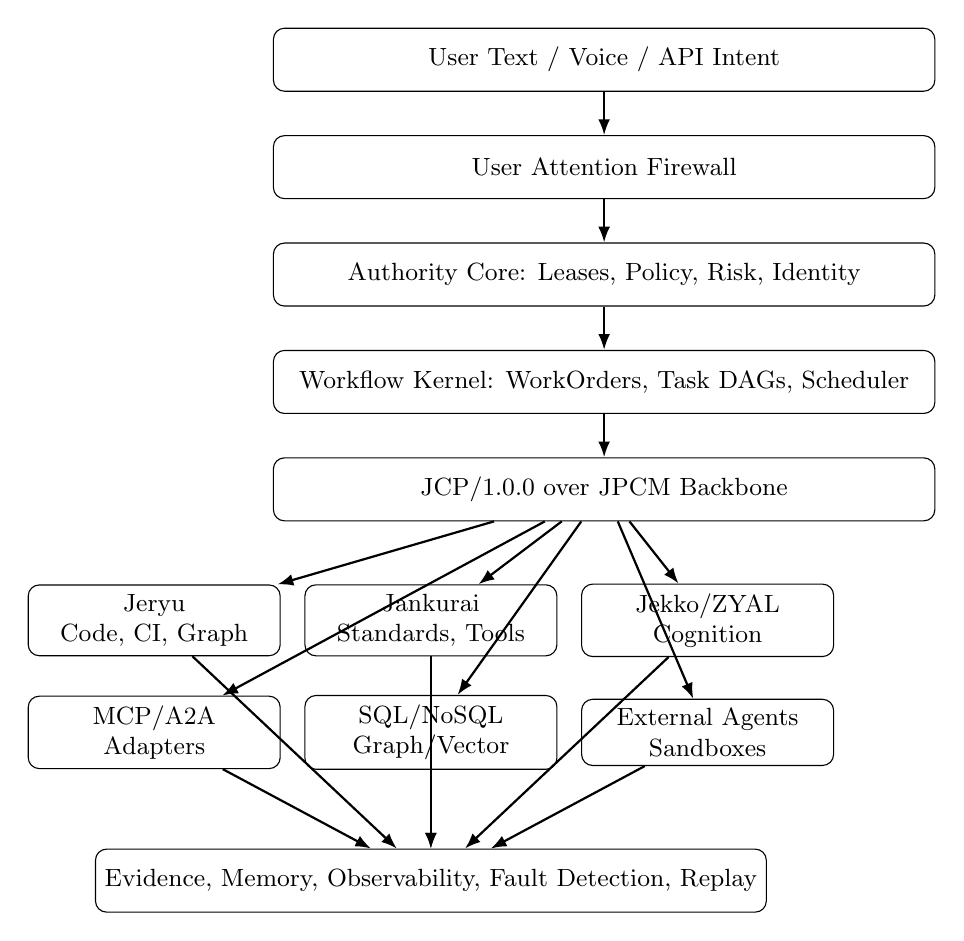
\begin{tikzpicture}[node distance=0.55cm, every node/.style={font=\small}, box/.style={draw, rounded corners, align=center, minimum width=3.2cm, minimum height=0.8cm}, wide/.style={draw, rounded corners, align=center, minimum width=8.4cm, minimum height=0.8cm}, arrow/.style={-{Latex[length=2mm]}, thick}]
\node[wide] (user) {User Text / Voice / API Intent};
\node[wide, below=of user] (attention) {User Attention Firewall};
\node[wide, below=of attention] (authority) {Authority Core: Leases, Policy, Risk, Identity};
\node[wide, below=of authority] (workflow) {Workflow Kernel: WorkOrders, Task DAGs, Scheduler};
\node[wide, below=of workflow] (jcp) {JCP/1.0.0 over JPCM Backbone};
\node[box, below left=0.8cm and -0.1cm of jcp] (jeryu) {Jeryu\\Code, CI, Graph};
\node[box, right=0.3cm of jeryu] (jank) {Jankurai\\Standards, Tools};
\node[box, right=0.3cm of jank] (jekko) {Jekko/ZYAL\\Cognition};
\node[box, below=0.5cm of jeryu] (mcp) {MCP/A2A\\Adapters};
\node[box, right=0.3cm of mcp] (data) {SQL/NoSQL\\Graph/Vector};
\node[box, right=0.3cm of data] (agents) {External Agents\\Sandboxes};
\node[wide, below=1.0cm of data] (evidence) {Evidence, Memory, Observability, Fault Detection, Replay};
\draw[arrow] (user) -- (attention);
\draw[arrow] (attention) -- (authority);
\draw[arrow] (authority) -- (workflow);
\draw[arrow] (workflow) -- (jcp);
\draw[arrow] (jcp) -- (jeryu);
\draw[arrow] (jcp) -- (jank);
\draw[arrow] (jcp) -- (jekko);
\draw[arrow] (jcp) -- (mcp);
\draw[arrow] (jcp) -- (data);
\draw[arrow] (jcp) -- (agents);
\draw[arrow] (jeryu) -- (evidence);
\draw[arrow] (jank) -- (evidence);
\draw[arrow] (jekko) -- (evidence);
\draw[arrow] (mcp) -- (evidence);
\draw[arrow] (data) -- (evidence);
\draw[arrow] (agents) -- (evidence);
\end{tikzpicture}
\caption{JMCP reference architecture. Authority, workflow, communication, evidence, and user attention are separate planes.}
\label{fig:arch}
\end{figure}

\subsection{Authority Core}
The Authority Core issues and revokes CapabilityLeases. It evaluates policy, risk tier, autonomy tier, data classification, budget, sandbox class, and user approval requirements. No service, tool, or agent may grant itself authority.

\subsection{Workflow Kernel}
The Workflow Kernel transforms intent into WorkOrders and Tasks. It manages state transitions, task DAGs, priorities, scheduling, retries, cancellation, quarantine, rollback, and promotion.

\subsection{Evidence Kernel}
The Evidence Kernel collects and evaluates EvidenceBundles. It maps evidence to claims, preserves negative evidence, detects conflicts, and refuses promotion when proof is insufficient.

\subsection{Attention Firewall}
The Attention Firewall decides what the user sees. Its task is not to hide work; it is to compress operational detail into the minimum useful packet while escalating material decisions.

\section{JCP/1.0.0 Protocol}
JCP/1.0.0 is the mandatory protocol for all communication with JMCP. It is stricter than a general event format because it carries authority, policy, trace, risk, data, and evidence context. A JCP message is a signed envelope with a typed payload.

\subsection{Envelope}
The required fields are `jcp\_version', `kind', `message\_id', `message\_type', `producer', `subject', `time', `trace', `authority', `policy', `data', `payload\_hash', `payload', and `signature'. Recommended fields include `ordering', `delivery', `risk', `attention', `evidence\_refs', `attachments', `redaction', and `encryption'.

\begin{lstlisting}[caption={Illustrative JCP/1.0.0 envelope.}]
{
  "jcp_version": "1.0.0",
  "kind": "JCPEnvelope",
  "message_id": "01JCP7P0F7S6V6K3M8QA3G2B4V",
  "message_type": "tool.call.requested",
  "subject": {"type":"task", "id":"task_123"},
  "time": "2026-06-01T17:30:00Z",
  "producer": {
    "service_id":"jmcp-workflow",
    "service_instance_id":"cell-a-42",
    "service_version":"1.0.0",
    "service_card_hash":"sha256:..."
  },
  "trace": {
    "trace_id":"trace_abc",
    "correlation_id":"work_789",
    "idempotency_key":"tool-call-task_123-attempt_1"
  },
  "authority": {
    "lease_id":"lease_456",
    "authority_class":"write_repo",
    "permissions":["repo.branch.write"],
    "scope":["repo:neverhuman/jeryu", "branch:jmcp/task_123"],
    "expires_at":"2026-06-01T17:45:00Z"
  },
  "policy": {"policy_epoch":"pe_2026_06_01", "decision_id":"pd_42"},
  "data": {"classification":"internal", "retention":"audit", "allowed_uses":["execution"]},
  "payload_hash":"sha256:...",
  "payload": {"command_id":"cmd_1", "command_type":"tool_call", "target":"jeryu.git", "requested_action":"create_branch"},
  "signature": {"alg":"ed25519", "kid":"jmcp-workflow#2026-06", "value":"...", "signed_at":"2026-06-01T17:30:00Z"}
}
\end{lstlisting}

\subsection{Message Families}
JCP/1.0.0 defines intent, work order, task, command, lease, context, tool, data, agent, evidence, policy, promotion, attention, voice, memory, self-improvement, tool-build, fault, telemetry, service, audit, conformance, and governance families. The family list is intentionally broad. It must cover normal software tasks, self-improvement, automated tool construction, data governance, and emergency control.

\subsection{Delivery Classes}
JCP does not assume exactly-once delivery. It uses idempotency, per-subject ordering, replay, and signatures. Delivery classes include ephemeral, durable-at-least-once, durable-ordered, command-requires-ack, and audit-append-only.

\subsection{Versioning}
JCP follows semantic versioning. Unknown non-critical fields may be ignored. Unknown critical fields fail closed. Services advertise supported versions in ServiceCards. A major protocol change is itself a governed WorkOrder.

\section{JPCM Communication Backbone}
JPCM is the default communication backbone profile. It carries JCP envelopes across durable event streams, request/reply, replay, and interactive channels. The recommended first implementation uses NATS JetStream for low-latency subject-based streams and request/reply, with optional Redpanda/Kafka for high-volume analytics. The backbone must support durable streams, poison-message quarantine, dead-letter queues, schema registry, envelope signature verification, backpressure, replay, tenant/cell isolation, and immutable audit streams.

During partitions, services degrade to safe mode. No new high-risk lease may be issued without authority quorum. Read-only cached views may continue with stale-data warnings. This is essential because an autonomous system that continues high-risk work while disconnected from authority has already lost the control-plane property.

\section{Service, Tool, Data, and Agent Cards}
Every participant must publish a signed ServiceCard before receiving authority. ToolCard, DataCard, and AgentCard extend this discovery model.

\begin{longtable}{p{0.18\linewidth}p{0.74\linewidth}}
\caption{Card types in JCP/1.0.0.}\label{tab:cards}\\
\toprule
Card & Required purpose \\
\midrule
\endfirsthead
\toprule
Card & Required purpose \\
\midrule
\endhead
ServiceCard & Identifies a service, version, owner, endpoints, transport profiles, capabilities, supported JCP versions, sandbox class, SBOM, attestations, SLOs, cost model, conformance level, and revocation subject. \\
ToolCard & Identifies a callable tool, input and output schemas, risk tier, side-effect class, required permissions, egress policy, test suite, owner, and evidence expectations. \\
DataCard & Identifies a data source, owner, classification, schema, retention, allowed uses, lineage, freshness SLO, redaction policy, and access constraints. \\
AgentCard & Identifies an agent or model runtime, provider, capabilities, context policy, sandbox requirement, risk limits, maximum autonomy tier, and evaluation references. \\
\bottomrule
\end{longtable}

A stale or unsigned card does not merely reduce confidence; it removes authority. Card publication and revocation are audit events.

\section{Capability Leases}
CapabilityLeases are the core authority primitive. A lease specifies who may do what, where, for how long, under what risk ceiling, with which data classes, budgets, egress permissions, sandbox class, and required evidence. Leases are checked at every side-effect boundary: context grant, tool call, data query, file write, git operation, CI operation, network egress, deployment, memory write, policy change, tool build, and self-improvement promotion.

\begin{figure}[!ht]
\centering
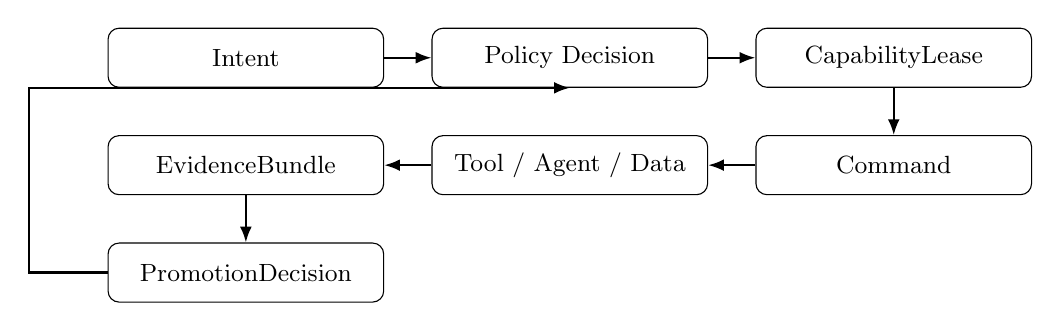
\begin{tikzpicture}[node distance=0.6cm, every node/.style={font=\small}, box/.style={draw, rounded corners, align=center, minimum width=3.5cm, minimum height=0.75cm}, arrow/.style={-{Latex[length=2mm]}, thick}]
\node[box] (intent) {Intent};
\node[box, right=of intent] (policy) {Policy Decision};
\node[box, right=of policy] (lease) {CapabilityLease};
\node[box, below=of lease] (command) {Command};
\node[box, left=of command] (tool) {Tool / Agent / Data};
\node[box, left=of tool] (evidence) {EvidenceBundle};
\node[box, below=of evidence] (promotion) {PromotionDecision};
\draw[arrow] (intent) -- (policy);
\draw[arrow] (policy) -- (lease);
\draw[arrow] (lease) -- (command);
\draw[arrow] (command) -- (tool);
\draw[arrow] (tool) -- (evidence);
\draw[arrow] (evidence) -- (promotion);
\draw[arrow] (promotion.west) -- ++(-1,0) |- (policy.south);
\end{tikzpicture}
\caption{Authority and evidence loop. Authority is leased before command execution; evidence gates promotion and may update policy.}
\label{fig:lease-loop}
\end{figure}

\section{Work Orders and Task Lifecycle}
An Intent is a user's or system's statement of desired outcome. A WorkOrder is the governed unit of value created from an intent. A Task is a typed node in a WorkOrder DAG. Task kinds include research, planning, coding, code review, test generation, CI triage, bug fix, refactor, security review, dependency update, release, deployment, incident response, observability analysis, data query, knowledge compression, memory maintenance, tool inventory, tool build, self-improvement, policy update, documentation, user communication, voice command, external agent delegation, governance, cost optimization, architecture design, experiment, benchmark, conformance test, backup/restore, migration, and legal/compliance.

\begin{figure}[!ht]
\centering
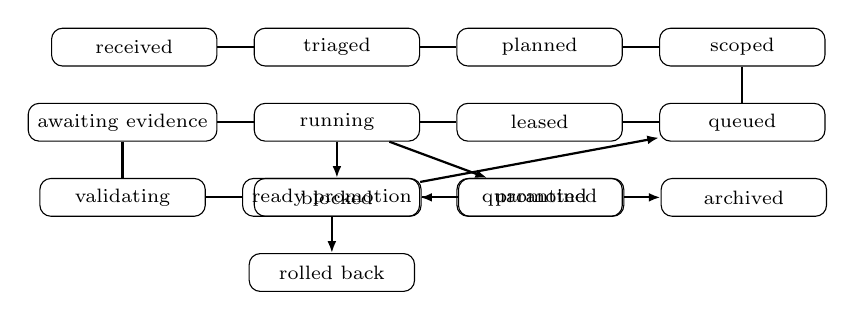
\begin{tikzpicture}[node distance=0.46cm, every node/.style={font=\scriptsize}, state/.style={draw, rounded corners, align=center, minimum width=2.1cm, minimum height=0.48cm}, arrow/.style={-{Latex[length=1.5mm]}, thick}]
\node[state] (received) {received};
\node[state, right=of received] (triaged) {triaged};
\node[state, right=of triaged] (planned) {planned};
\node[state, right=of planned] (scoped) {scoped};
\node[state, below=of scoped] (queued) {queued};
\node[state, left=of queued] (leased) {leased};
\node[state, left=of leased] (running) {running};
\node[state, left=of running] (evidence) {awaiting evidence};
\node[state, below=of evidence] (validating) {validating};
\node[state, right=of validating] (ready) {ready promotion};
\node[state, right=of ready] (promoted) {promoted};
\node[state, right=of promoted] (archived) {archived};
\node[state, below=of running] (blocked) {blocked};
\node[state, below=of leased] (quarantine) {quarantined};
\node[state, below=of ready] (rollback) {rolled back};
\draw[arrow] (received)--(triaged)--(planned)--(scoped)--(queued)--(leased)--(running)--(evidence)--(validating)--(ready)--(promoted)--(archived);
\draw[arrow] (running)--(blocked);
\draw[arrow] (blocked)--(queued);
\draw[arrow] (running)--(quarantine);
\draw[arrow] (ready)--(rollback);
\draw[arrow] (quarantine)--(blocked);
\end{tikzpicture}
\caption{Canonical task lifecycle. Illegal transitions are rejected and recorded as faults.}
\label{fig:task-state}
\end{figure}

A task may be blocked, quarantined, retried, paused, canceled, rejected, or rolled back. Every non-read-only task must either have a rollback plan or be marked irreversible. Irreversible actions require explicit attention unless covered by emergency policy.

\section{Evidence and Promotion}
Evidence is not logs. Logs are raw material. Evidence is a claim-supporting artifact bundle. An EvidenceBundle includes evidence class, items, summary, sufficiency, supported claims, unsupported claims, reproducer, provenance, and negative evidence. PromotionDecision objects approve, reject, quarantine, or request more evidence.

\begin{longtable}{p{0.18\linewidth}p{0.74\linewidth}}
\caption{Evidence sufficiency levels.}\label{tab:evidence}\\
\toprule
Level & Meaning \\
\midrule
\endfirsthead
\toprule
Level & Meaning \\
\midrule
\endhead
insufficient & Evidence does not support the claimed result. \\
partial & Evidence supports some claims but not enough for review or promotion. \\
sufficient for review & Evidence is enough for human or independent review, not autonomous promotion. \\
sufficient for promotion & Evidence satisfies the task's risk-specific promotion gate. \\
conflicting & Evidence contains unresolved contradictions and blocks promotion. \\
\bottomrule
\end{longtable}

High-risk work requires independent evidence. The worker that changed code should not be the only verifier that the change is safe. This is especially important for security, deployment, dependency, and self-improvement tasks.

\section{User Attention Firewall}
JMCP's user interface should protect the user from operational flood. This is not the same as hiding information. The Attention Firewall translates internal state into minimal useful packets: silent, digest, notify, ask, interrupt, block-until-user, and emergency.

\begin{figure}[!ht]
\centering
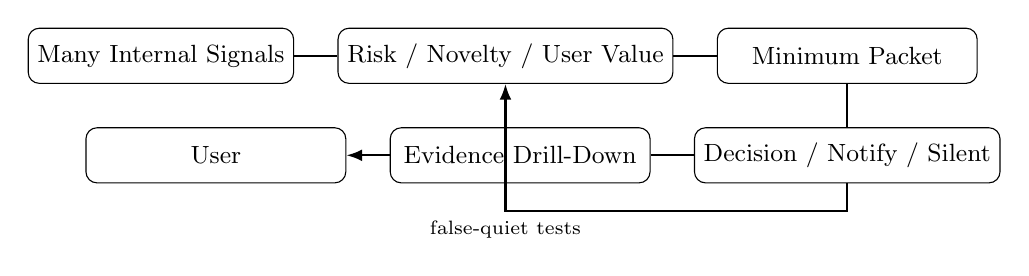
\begin{tikzpicture}[node distance=0.55cm, every node/.style={font=\small}, box/.style={draw, rounded corners, align=center, minimum width=3.3cm, minimum height=0.7cm}, arrow/.style={-{Latex[length=2mm]}, thick}]
\node[box] (signals) {Many Internal Signals};
\node[box, right=of signals] (classify) {Risk / Novelty / User Value};
\node[box, right=of classify] (compress) {Minimum Packet};
\node[box, below=of compress] (decision) {Decision / Notify / Silent};
\node[box, left=of decision] (drill) {Evidence Drill-Down};
\node[box, left=of drill] (user) {User};
\draw[arrow] (signals)--(classify)--(compress)--(decision)--(drill)--(user);
\draw[arrow] (decision.south) -- ++(0,-0.35) -| node[below,font=\scriptsize]{false-quiet tests} (classify.south);
\end{tikzpicture}
\caption{Attention Firewall. The system compresses operational detail while preserving drill-down and mandatory escalation.}
\label{fig:attention}
\end{figure}

Mandatory escalation occurs when risk tier rises, cost budget will be exceeded, data classification escalates, credential access is requested, public or external communication is requested, production deployment is requested, irreversible change is requested, evidence conflicts, intent is uncertain, policy exception is requested, self-improvement affects authority/evidence/memory/routing, or a false-quiet check fails.

\section{Text and Voice Interfaces}
Text remains the highest-fidelity user channel. Voice is supported for fast interaction, status queries, task creation, and decision confirmation. However, voice is a security boundary. A VoiceTurn includes session id, speaker id, audio reference, transcript, confidence, command candidate flag, confirmation requirement, anti-replay nonce, and ambient-context warning.

No irreversible R4+ action may be authorized through ambiguous voice alone. The system must preserve transcript and confirmation evidence. Voice commands may create WorkOrders, request status, ask for summaries, or approve low-risk reversible actions within policy. Higher-risk actions require explicit confirmation and may require text review.

\section{Tool and Data Awareness}
JMCP must be tool and data aware. It maintains a capability graph covering services, tools, agents, models, data stores, repositories, tests, CI jobs, policies, owners, costs, SLOs, credentials, known failures, and evidence history. Tool and data awareness is not a static catalog. It is a living operational model used for scheduling, routing, risk scoring, and improvement.

The Technology Scout loop asks whether repeated pain should become a reusable tool. The system should know what technologies it has, what technologies are weak, what tools are missing, what should be built, and whether a new tool belongs locally, in Jankurai, or in a broader registry.

\section{Automated Tool Building}
Automated tool building is first-class. A ToolBuildProposal records the problem, intended users, risk tier, spec reference, implementation repository, evaluation plan, quarantine period, and publish target. The workflow is detect, propose, specify, implement in sandbox, test, fuzz, red-team, shadow, quarantine, promote, monitor, and deprecate if needed.

A tool that affects code, data, secrets, external systems, money, or deployments cannot be promoted solely by the agent that built it. It requires independent evidence and promotion decision. Global tools are published to Jankurai only after cross-repo generality and safety are demonstrated.

\begin{figure}[!ht]
\centering
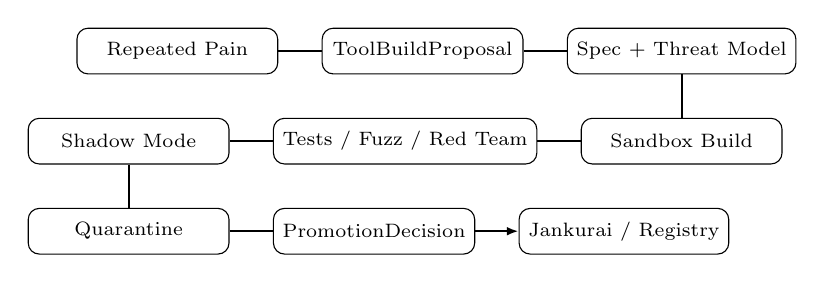
\begin{tikzpicture}[node distance=0.55cm, every node/.style={font=\scriptsize}, box/.style={draw, rounded corners, align=center, minimum width=2.55cm, minimum height=0.58cm}, arrow/.style={-{Latex[length=1.5mm]}, thick}]
\node[box] (pain) {Repeated Pain};
\node[box, right=of pain] (proposal) {ToolBuildProposal};
\node[box, right=of proposal] (spec) {Spec + Threat Model};
\node[box, below=of spec] (impl) {Sandbox Build};
\node[box, left=of impl] (tests) {Tests / Fuzz / Red Team};
\node[box, left=of tests] (shadow) {Shadow Mode};
\node[box, below=of shadow] (quarantine) {Quarantine};
\node[box, right=of quarantine] (promote) {PromotionDecision};
\node[box, right=of promote] (jankurai) {Jankurai / Registry};
\draw[arrow] (pain)--(proposal)--(spec)--(impl)--(tests)--(shadow)--(quarantine)--(promote)--(jankurai);
\end{tikzpicture}
\caption{Automated tool-building pipeline. New tools are products with evidence, not ad hoc scripts.}
\label{fig:toolbuild}
\end{figure}

\section{Memory and Knowledge Compression}
Memory is governed. The system does not write durable memory directly from model output. It creates MemoryProposals with source task, claim, scope, confidence, retention, contradiction checks, and review requirements. Memory can be accepted, rejected, decayed, contradicted, or scoped. Cross-repo lessons can be promoted into Jankurai when supported by evidence.

Knowledge compression is the conversion of noisy operational experience into reusable standards, tests, policies, workflows, and tools. The compression process is itself auditable. It must preserve enough provenance to explain why a lesson exists and when it should be retired.

\section{Self-Improvement}
JMCP should always improve, but safe improvement is a workflow. A SelfImprovementProposal includes target component, change summary, hypothesis, safety case, evaluation plan, shadow-mode requirement, rollback plan, and promotion gates. Self-improvement may target prompts, ZYAL workflows, scheduling heuristics, router rules, evidence requirements, memory policies, UI summarization, tests, and tool recommendations. It may not silently alter the authority kernel.

Forbidden unilateral changes include reducing evidence requirements, increasing autonomy tier, widening leases, weakening sandboxing, suppressing attention thresholds, changing policy semantics, altering audit retention, and changing identity trust roots. Such changes require governance workflows.

\section{Security Architecture}
JMCP's security architecture combines workload identity, signed envelopes, short-lived capability leases, policy-as-code, sandbox classes, egress control, secret brokering, provenance, immutable audit logs, conformance tests, watchdog veto, and break-glass audit. It follows zero-trust principles: location does not imply trust, and each resource access is authorized explicitly \cite{nistzt}.

The design directly addresses common agentic failure modes: prompt injection, tool poisoning, excessive agency, insecure tool output handling, data exfiltration, memory poisoning, confused deputy, sandbox escape, cost attack, and malicious delegation. A service that bypasses JCP is not merely incomplete; it is outside the trust boundary.

\section{Observability and Fault Detection}
JMCP must observe itself and all subordinate systems. Every envelope carries trace context. OpenTelemetry-compatible spans, metrics, and logs are emitted for tasks, tool calls, model calls, evidence generation, policy decisions, lease checks, voice interactions, and attention decisions. Fault detection covers SLO breach, cost breach, replay storm, schema drift, service degradation, evidence conflict, attention failure, and policy exceptions.

Observability is not enough by itself. The system must act on observations: degrade, quarantine, revoke leases, escalate to the user, rollback, or trigger incident workflow.

\section{Evaluation and Conformance}
Evaluation has three layers. First, protocol conformance tests validate schemas, signatures, idempotency, delivery classes, error handling, service cards, and lease enforcement. Second, adversarial tests attack prompt injection, tool poisoning, memory poisoning, voice spoofing, confused deputy, sandbox escape, data exfiltration, and cost denial-of-wallet. Third, operational tests measure user attention quality, evidence sufficiency, task success, rollback success, and learning value.

A conforming service reports bronze, silver, gold, or platinum conformance. Bronze means it validates envelopes and signs ServiceCards. Silver adds idempotency, leases, and schema compatibility. Gold adds evidence and replay. Platinum adds adversarial test results, provenance, and fault-injection results.

\section{Implementation Blueprint}
The recommended implementation stack is Rust for core services, Tokio/Axum/tonic for async networking, NATS JetStream for JPCM, PostgreSQL for authority and task state, object/CAS store for evidence, graph store for capability and code relationships, vector/search index for retrieval, OpenTelemetry for observability, and Vite/TypeScript/React for the cockpit. WebRTC carries voice media; signed JCP envelopes carry voice control semantics.

The repository should contain generated Rust and TypeScript bindings for JCP/1.0.0, validators, authority core, workflow kernel, evidence kernel, memory kernel, attention firewall, tool registry, tool builder, self-improvement engine, backbone adapters, observability, security, and adapters for Jankurai, Jeryu, Jekko/ZYAL, MCP, A2A, GitHub, SQL, NoSQL, graph, vector, and voice.

\section{Extreme Future Vector}
JMCP's near-term role is an engineering command room. Its long-term vector is much larger.

At Horizon 1, JMCP becomes the single interface for repositories, CI, issues, logs, tasks, agents, and lessons. At Horizon 2, it becomes an autonomous engineering fab that continuously finds bugs, reduces redundancy, improves tests, updates dependencies, and builds tools. At Horizon 3, it becomes a cross-repository process-yield optimizer. At Horizon 4, it becomes an engineering digital twin: a live model of code, tools, data, risk, cost, defects, delivery flow, and knowledge. At Horizon 5, it becomes an autonomous R\&D foundry that searches, hypothesizes, prototypes, tests, compresses knowledge, and retires weak ideas. At Horizon 6, it becomes a proof-carrying agent economy where agents compete by producing evidence-carrying work. At Horizon 7, it becomes a federated control-plane mesh that exchanges signed lessons, tools, and trust without exposing private data. At Horizon 8, it becomes a cognitive process-control operating system.

This ambition is not a license to weaken controls. It is the reason controls must be stronger. The more capable JMCP becomes, the more strictly it must govern authority, evidence, memory, and attention.

\section{Limitations and Residual Critique}
No design is literally beyond critique. Several problems remain open. Formal verification of policy composition is hard. Measuring evidence sufficiency for creative work is hard. Preventing benchmark gaming in self-improvement is hard. Calibrating user trust without over-notifying is hard. Building universal tool and data awareness without stale metadata is hard. Federated trust exchange without leaking private information is hard. These problems must remain visible in the roadmap rather than hidden in marketing claims.

\section{Conclusion}
JMCP is strongest when it is not imagined as a smarter agent. It is a control plane that governs agents, tools, data, memory, evidence, and user attention. JCP/1.0.0 is the final mandatory protocol that makes that control plane buildable. The architecture's central claim is simple: autonomous engineering becomes safer and more valuable not by granting agents more ambient autonomy, but by giving every action a typed task, every side effect a lease, every promotion evidence, every memory a proposal, every service a signed card, and every user interruption a reason.

\appendices

\section{Normative Message Families}
\begin{longtable}{p{0.22\linewidth}p{0.68\linewidth}}
\toprule
Family & Normative role \\
\midrule
intent & Intake of user, API, scheduled, or system intent. \\
work\_order & Governed unit of value with objective, owner, budgets, tasks, and evidence requirements. \\
task & Task creation, transition, blocking, retry, quarantine, promotion, rejection, rollback, and archival. \\
command & Request/result lifecycle for tools, data, agents, repo changes, CI, deployment, user messages, and voice confirmations. \\
lease & Request, issue, renew, revoke, expire, and violation of capability authority. \\
context & Context request, grant, denial, expiration, and redaction. \\
tool & Tool card publication and tool call lifecycle. \\
data & Data card publication, query lifecycle, access denial, lineage update. \\
agent & Agent card publication and delegation lifecycle. \\
evidence & Evidence append, rejection, sufficiency assessment, and conflict detection. \\
policy & Policy decision, epoch publication, exceptions, and veto. \\
promotion & Request, approval, rejection, and revocation of work promotion. \\
attention & User attention packets, escalations, resolutions, and false-quiet alarms. \\
voice & Voice segment, transcript, command candidate, confirmation, and rejection. \\
memory & Memory proposal, acceptance, rejection, decay, and contradiction. \\
self\_improvement & Proposal, approval, shadow mode, evaluation, promotion, and reversion. \\
tool\_build & Proposal, specification, implementation, testing, quarantine, promotion, and deprecation. \\
fault & Detection, triage, mitigation, postmortem, and watchdog veto. \\
telemetry & Metric, SLO breach, and cost breach events. \\
service & Service card publication, heartbeat, health, degradation, and decommissioning. \\
audit & Append-only audit records. \\
conformance & Protocol conformance reports. \\
governance & Protocol freeze, vote, and major change events. \\
\bottomrule
\end{longtable}

\section{Risk and Autonomy Tiers}
\begin{longtable}{p{0.18\linewidth}p{0.32\linewidth}p{0.38\linewidth}}
\toprule
Tier & Meaning & Default user policy \\
\midrule
R0 & Observe only & Silent or digest. \\
R1 & Read-only & Silent unless sensitive data is accessed. \\
R2 & Local reversible & Notify or silent depending on history. \\
R3 & Repository write & Evidence required, user may review. \\
R4 & External side effect & Ask or block depending on scope. \\
R5 & Security-sensitive & Block until evidence and approval. \\
R6 & Financial or legal & Explicit user approval. \\
R7 & Irreversible or public & Explicit approval and rollback/mitigation plan. \\
\bottomrule
\end{longtable}

\section{Final Acceptance Checklist}
A build is not accepted until all items hold: every service speaks JCP/1.0.0 or sits behind a conforming adapter; the schema validates all core payload types; no side-effecting command executes without a lease; illegal task transitions are rejected; evidence bundles are required for promotion; the user can drill from summary to evidence; voice commands produce transcripts and confirmation artifacts; self-improvement cannot mutate authority without governance; tool-building outputs are quarantined until independent evidence passes; a full task can be replayed; conformance failures revoke authority; false-quiet tests detect under-notification; budgets are enforced; memory proposals can be contradicted or decayed; and break-glass incidents produce user-visible audit artifacts.

\begin{thebibliography}{60}
\bibitem{mcp2025} Model Context Protocol, ``Specification, Version 2025-06-18,'' 2025. [Online]. Available: \url{https://modelcontextprotocol.io/specification/2025-06-18}
\bibitem{a2a2026} A2A Protocol Project, ``Agent2Agent Protocol Specification,'' 2026. [Online]. Available: \url{https://a2a-protocol.org/latest/specification/}
\bibitem{owaspllm} OWASP Foundation, ``OWASP Top 10 for Large Language Model Applications,'' 2025. [Online]. Available: \url{https://owasp.org/www-project-top-10-for-large-language-model-applications/}
\bibitem{owaspagentic} OWASP Foundation, ``Agentic AI Security Initiative,'' 2025. [Online]. Available: \url{https://genai.owasp.org/}
\bibitem{nistai} NIST, ``Artificial Intelligence Risk Management Framework (AI RMF 1.0),'' 2023. [Online]. Available: \url{https://www.nist.gov/itl/ai-risk-management-framework}
\bibitem{nistzt} S. Rose, O. Borchert, S. Mitchell, and S. Connelly, ``Zero Trust Architecture,'' NIST SP 800-207, 2020. [Online]. Available: \url{https://doi.org/10.6028/NIST.SP.800-207}
\bibitem{nistssdf} M. Souppaya, K. Scarfone, and D. Dodson, ``Secure Software Development Framework (SSDF) Version 1.1,'' NIST SP 800-218, 2022. [Online]. Available: \url{https://doi.org/10.6028/NIST.SP.800-218}
\bibitem{nist80053} NIST, ``Security and Privacy Controls for Information Systems and Organizations,'' SP 800-53 Rev. 5, 2020. [Online]. Available: \url{https://doi.org/10.6028/NIST.SP.800-53r5}
\bibitem{nistcsf} NIST, ``The NIST Cybersecurity Framework 2.0,'' 2024. [Online]. Available: \url{https://www.nist.gov/cyberframework}
\bibitem{slsa} OpenSSF, ``Supply-chain Levels for Software Artifacts (SLSA),'' 2026. [Online]. Available: \url{https://slsa.dev/}
\bibitem{in_toto} in-toto Project, ``A framework to secure the integrity of software supply chains,'' 2026. [Online]. Available: \url{https://in-toto.io/}
\bibitem{sigstore} Sigstore Project, ``Sigstore: Software signing for everybody,'' 2026. [Online]. Available: \url{https://www.sigstore.dev/}
\bibitem{tuf} The Update Framework, ``Specification,'' 2026. [Online]. Available: \url{https://theupdateframework.io/}
\bibitem{spdx} Linux Foundation, ``SPDX Specification,'' 2026. [Online]. Available: \url{https://spdx.dev/}
\bibitem{cyclonedx} OWASP Foundation, ``CycloneDX Software Bill of Materials Standard,'' 2026. [Online]. Available: \url{https://cyclonedx.org/}
\bibitem{spiffe} SPIFFE Project, ``SPIFFE Overview,'' 2026. [Online]. Available: \url{https://spiffe.io/docs/latest/spiffe-about/overview/}
\bibitem{spire} SPIRE Project, ``SPIRE Documentation,'' 2026. [Online]. Available: \url{https://spiffe.io/docs/latest/spire-about/}
\bibitem{otel} OpenTelemetry, ``OpenTelemetry Specification,'' 2026. [Online]. Available: \url{https://opentelemetry.io/docs/specs/}
\bibitem{otelgenai} OpenTelemetry, ``Semantic conventions for generative AI systems,'' 2026. [Online]. Available: \url{https://opentelemetry.io/docs/specs/semconv/gen-ai/}
\bibitem{cloudevents} CloudEvents, ``CloudEvents Specification,'' 2026. [Online]. Available: \url{https://cloudevents.io/}
\bibitem{jsonschema} JSON Schema Organization, ``JSON Schema Draft 2020-12,'' 2020. [Online]. Available: \url{https://json-schema.org/draft/2020-12}
\bibitem{jsonrpc} JSON-RPC Working Group, ``JSON-RPC 2.0 Specification,'' 2013. [Online]. Available: \url{https://www.jsonrpc.org/specification}
\bibitem{rfc2119} S. Bradner, ``Key words for use in RFCs to Indicate Requirement Levels,'' RFC 2119, 1997.
\bibitem{rfc8174} B. Leiba, ``Ambiguity of Uppercase vs Lowercase in RFC 2119 Key Words,'' RFC 8174, 2017.
\bibitem{rfc9110} R. Fielding, M. Nottingham, and J. Reschke, ``HTTP Semantics,'' RFC 9110, 2022.
\bibitem{rfc8446} E. Rescorla, ``The Transport Layer Security (TLS) Protocol Version 1.3,'' RFC 8446, 2018.
\bibitem{oauth2} D. Hardt, ``The OAuth 2.0 Authorization Framework,'' RFC 6749, 2012.
\bibitem{oidc} OpenID Foundation, ``OpenID Connect Core 1.0,'' 2014. [Online]. Available: \url{https://openid.net/specs/openid-connect-core-1_0.html}
\bibitem{opa} Open Policy Agent, ``OPA Documentation,'' 2026. [Online]. Available: \url{https://www.openpolicyagent.org/docs/latest/}
\bibitem{nats} NATS.io, ``NATS JetStream Documentation,'' 2026. [Online]. Available: \url{https://docs.nats.io/nats-concepts/jetstream}
\bibitem{kafka} J. Kreps, N. Narkhede, and J. Rao, ``Kafka: A Distributed Messaging System for Log Processing,'' NetDB, 2011.
\bibitem{raft} D. Ongaro and J. Ousterhout, ``In Search of an Understandable Consensus Algorithm,'' USENIX ATC, 2014.
\bibitem{lamport} L. Lamport, ``Time, Clocks, and the Ordering of Events in a Distributed System,'' Commun. ACM, 1978.
\bibitem{byzantine} L. Lamport, R. Shostak, and M. Pease, ``The Byzantine Generals Problem,'' ACM TOPLAS, 1982.
\bibitem{flp} M. Fischer, N. Lynch, and M. Paterson, ``Impossibility of Distributed Consensus with One Faulty Process,'' J. ACM, 1985.
\bibitem{cap} E. Brewer, ``CAP Twelve Years Later: How the Rules Have Changed,'' Computer, 2012.
\bibitem{sre} B. Beyer, C. Jones, J. Petoff, and N. Murphy, ``Site Reliability Engineering,'' O'Reilly, 2016.
\bibitem{accelerate} N. Forsgren, J. Humble, and G. Kim, ``Accelerate,'' IT Revolution, 2018.
\bibitem{openapi} OpenAPI Initiative, ``OpenAPI Specification,'' 2026. [Online]. Available: \url{https://spec.openapis.org/}
\bibitem{asyncapi} AsyncAPI Initiative, ``AsyncAPI Specification,'' 2026. [Online]. Available: \url{https://www.asyncapi.com/docs/reference/specification/latest}
\bibitem{webrtc} W3C, ``WebRTC: Real-Time Communication in Browsers,'' 2025. [Online]. Available: \url{https://www.w3.org/TR/webrtc/}
\bibitem{webspeech} W3C, ``Web Speech API,'' 2025. [Online]. Available: \url{https://webaudio.github.io/web-speech-api/}
\bibitem{tla} L. Lamport, ``Specifying Systems: The TLA+ Language and Tools for Hardware and Software Engineers,'' Addison-Wesley, 2002.
\bibitem{stpa} N. Leveson, ``Engineering a Safer World,'' MIT Press, 2011.
\bibitem{nist160} NIST, ``Systems Security Engineering,'' SP 800-160 Vol. 1 Rev. 1, 2022.
\bibitem{cwe} MITRE, ``Common Weakness Enumeration,'' 2026. [Online]. Available: \url{https://cwe.mitre.org/}
\bibitem{attack} MITRE, ``ATT\&CK Framework,'' 2026. [Online]. Available: \url{https://attack.mitre.org/}
\bibitem{atlas} MITRE, ``ATLAS: Adversarial Threat Landscape for Artificial-Intelligence Systems,'' 2026. [Online]. Available: \url{https://atlas.mitre.org/}
\bibitem{oci} Open Container Initiative, ``Runtime and Image Specifications,'' 2026. [Online]. Available: \url{https://opencontainers.org/}
\bibitem{wasi} Bytecode Alliance, ``WebAssembly System Interface,'' 2026. [Online]. Available: \url{https://wasi.dev/}
\bibitem{wasmtime} Bytecode Alliance, ``Wasmtime,'' 2026. [Online]. Available: \url{https://wasmtime.dev/}
\bibitem{owaspasvs} OWASP Foundation, ``Application Security Verification Standard,'' 2026. [Online]. Available: \url{https://owasp.org/www-project-application-security-verification-standard/}
\bibitem{owaspsamm} OWASP Foundation, ``Software Assurance Maturity Model,'' 2026. [Online]. Available: \url{https://owasp.org/www-project-samm/}
\bibitem{invariantmcp} Invariant Labs, ``MCP Security Notification: Tool Poisoning Attacks,'' 2025. [Online]. Available: \url{https://invariantlabs.ai/}
\bibitem{houmcp} X. Hou, Y. Zhao, S. Wang, and H. Wang, ``Model Context Protocol (MCP): Landscape, Security Threats, and Future Research Directions,'' 2025.
\bibitem{krawiecka} K. Krawiecka and C. Schroeder de Witt, ``Extending the OWASP Multi-Agentic System Threat Modeling Guide,'' 2025.
\bibitem{saga} M. D. Laws, A. Oprea, and C. Nita-Rotaru, ``Attacks and Mitigations for Distributed Governance of Agentic AI under Byzantine Adversaries,'' 2026.
\bibitem{gomez} F. Gomez, ``Adapting Insider Risk Mitigations for Agentic Misalignment,'' 2025.
\bibitem{lewis} M. Lewis, P. Marinescu, and M. Fowler, ``Microservices Resource Guide,'' 2014. [Online]. Available: \url{https://martinfowler.com/microservices/}
\bibitem{eventsource} M. Fowler, ``Event Sourcing,'' 2005. [Online]. Available: \url{https://martinfowler.com/eaaDev/EventSourcing.html}
\bibitem{rfc6902} P. Bryan and M. Nottingham, ``JavaScript Object Notation (JSON) Patch,'' RFC 6902, 2013.
\bibitem{rfc8785} A. Rundgren, B. Jordan, and S. Erdtman, ``JSON Canonicalization Scheme,'' RFC 8785, 2020.
\bibitem{uuid} K. Davis and B. Peabody, ``Universally Unique IDentifiers (UUIDs),'' RFC 9562, 2024.
\end{thebibliography}

\end{document}
